%% W11 (2026-11-10): rho with the refused ASKs put back, and the two margins reported apart.
%% Numbers: paper/cogsci2027/validation_20261108/results/w11_ask_refusal.json (rows: results/w11_ask_rows.csv),
%% written by paper/cogsci2027/validation_20261108/tools/w11_ask_refusal.py, which also writes the two tables
%% ko/parts/w11_tab_cells.tex, ko/parts/w11_tab_bands.tex and figures/w11_ask_refusal.{pdf,png}.
\subsection{두 가지 반론과 이 절의 결론}\label{val:w11-claims}

$\rho$에 대한 반론은 두 가지다. 하나는 토큰을 주지 않는 선택이 더 자기 보존적인 행동인데, $\rho$는 이전량 $g_k$로 가중하므로 거절에 가중치 0을 주어 그 선택을 보지 못한다는 것이다. 다른 하나는 비율로 묶으면 지원자가 어디까지 내려갔는지(분자)와 동료가 얼마나 채워졌는지(분모)가 섞인다는 것이다. 이 절은 두 반론을 모두 받아들인다. 요청을 거절한 결정을 다시 넣으면 네 상금 조건 모두에서 비율이 커졌으므로, GIVE만 보는 $\rho$는 결정 단위의 자기 쪽 여유 유지를 작게 잡는다. 분자와 분모를 나누어 보면 거절과 수락은 요청한 쪽의 여유에서는 거의 같았고 요청받은 쪽 자신의 여유에서 달랐다. 따라서 $\rho$의 크기만으로는 지원 결정이 자기 여유를 따랐는지 동료의 부족을 따랐는지 알 수 없다. 두 결과 모두 $\rho$를 자기 보존 지표로 쓰지 않는다는 절~\ref{val:w2-rho}의 결론을 바꾸지 않고, 모델 비교에는 거절 빈도와 두 여유를 따로 적어야 한다는 요구를 더한다.

\subsection{표본: ASK를 받은 뒤의 첫 결정}\label{val:w11-sample}

표본은 실행된 ASK 하나하나에서 시작한다. 네 상금 조건 200판의 ASK 697건 가운데, 같은 판·라운드에서 같은 요청자가 같은 상대에게 처음 보낸 ASK 595건을 분석 단위로 삼아 반복 요청을 한 번만 셌다. 요청받은 에이전트의 응답은 그 ASK보다 늦은 tick의 첫 TALK 호출이다. 같은 tick의 호출은 동시에 생성되므로 그 ASK를 볼 수 없다. 이 응답이 없거나 그때 요청자가 이미 빠진 5건을 빼면 590건이 남는다. 결과는 요청받은 쪽이 그 라운드에서 요청자에게 실제로 실행한 GIVE로 나누었다. 첫 응답의 GIVE는 즉시 지원, 그 뒤의 GIVE는 지연 지원이고, 라운드가 끝날 때까지 GIVE가 없으면 거절이다. v33에는 거절 명령이 없으므로 거절은 GIVE하지 않은 응답을 뜻하며, 무응답(\texttt{DONE}만 쓴 응답)도 포함한다.

교차한 요청 119건은 거절에서 뺐다. 요청받은 쪽이 ASK 이전 또는 같은 tick에 이미 그 요청자에게 GIVE했고 ASK 뒤에는 더 주지 않은 경우다. 예를 들어 Opus 4107번 판 6라운드의 두 응답은 ``your message probably crossed with the transfers''라고 쓰고 이미 보낸 4,000토큰을 알렸다. 이 경우를 거절로 세면 본 실험에서 Opus의 거절 17건이 모두 교차였고, 거절과 수락을 가르는 변수가 요청자의 여유처럼 보였다. 교차를 뺀 결정은 471건이며, 즉시 지원 314건, 지연 지원 53건, 거절 104건(22\%)이다.

양쪽의 상태는 응답 tick이 시작할 때의 장부로 계산했다. 토큰 $b$는 응답 비용을 빼기 전 잔액이고, 생존 여유 $L=(b-\text{미납 벌금})/F_r$는 $\rho$와 같은 정의다. 결과 뒤 대화에서는 그 라운드의 확정 벌금을 빼고, 풀이 전 대화에서는 0을 뺐다. 결정 뒤 상태는 그 라운드에서 ASK 뒤에 실행된 GIVE 총량 $g$를 양쪽에 반영해 지원자 $L_s-g/F_r$, 요청자 $L_t+g/F_r$로 두었고, 거절은 두 여유를 그대로 둔다. 요청받은 쪽은 다른 에이전트의 잔액을 보지 못하고 토큰 순위와 자기 잔액, ASK 문구만 본다. 따라서 $L_t$와 토큰 비 $b_s/b_t$는 분석자가 장부로 계산한 값이며 응답자가 본 정보가 아니다. 불확실성은 모델·조건마다 열 시드를 블록으로 4,000회 다시 뽑은 백분위 95\% 구간이다.

\subsection{반론 1: 거절을 다시 넣은 비율}\label{val:w11-refusal}

거절은 거의 언제나 더 많이 가진 쪽의 선택이었다. 거절 104건 중 102건에서 요청받은 쪽의 토큰이 요청자보다 많았다. 요청자가 안전선 아래($L_t<1$)이고 요청받은 쪽이 요청자를 $L=1$까지 올린 뒤에도 자신은 $L\geq2$를 지킬 수 있던 182건으로 좁혀도 35건(19\%, 22판)이 거절이었다. 이 35건의 토큰 비 중앙값은 6.27로, 거절한 쪽이 요청자의 여섯 배 이상을 가지고 있었다. 이 가운데 13건에서는 같은 라운드에 다른 동료가 요청자에게 GIVE했으므로, 모든 거절을 요청자를 혼자 둔 결정으로 읽지는 않는다. 같은 조건에서 거절은 Fable 13건, Luna 12건, Sol 9건, Opus 1건이었고 Astra는 없었다.

\begin{table}[H]
\centering
\caption{ASK 뒤 결정과 양쪽 여유. 첫 ASK는 판·라운드·요청 쌍의 첫 요청 중 교차하지 않은 결정 수다. $\bar L_s$와 $\bar L_t$는 결정 직전 요청받은 쪽과 요청한 쪽의 평균 생존 여유이며, GIVE는 즉시·지연 지원, 거절은 라운드 안 GIVE가 없던 결정이다. 토큰 비는 결정 직전 $b_s/b_t$의 기하평균이다. $\rho_{\mathrm{GIVE}}$는 응답된 ASK만으로 계산한 이전량 가중 비율이고, $\rho_{\mathrm{all}}$은 거절을 포함한 모든 결정에서 결정 뒤 평균 $L_s$를 평균 $L_t$로 나눈 값이다. 괄호는 시드 블록 부트스트랩 4,000회 95\% 구간이다. 거절이 0건인 칸은 --로 두었다.}
\label{val:w11-tab-cells}
\resizebox{\linewidth}{!}{\begin{tabular}{lrcccccc}
\toprule
모델 & 첫 ASK & 즉시 / 지연 / 거절 & GIVE: $\bar L_s$ / $\bar L_t$ & 거절: $\bar L_s$ / $\bar L_t$ & 토큰 비 GIVE / 거절 & $\rho_{\mathrm{GIVE}}$ & $\rho_{\mathrm{all}}$ \\
\midrule
\multicolumn{8}{l}{2,000만 나눔(본 실험)} \\
Fable & 65 & 38 / 8 / 19 & 5.21 / 0.85 & 4.23 / 0.73 & 4.95 / 5.48 & 4.28 [3.74, 5.03] & 4.42 [3.78, 5.23] \\
Opus & 17 & 14 / 3 / 0 & 5.49 / 1.00 & -- / -- & 4.45 / -- & 2.68 [1.53, 7.00] & 3.26 [1.85, 7.82] \\
Astra & 9 & 7 / 0 / 2 & 6.26 / 0.96 & 4.72 / 1.96 & 3.68 / 2.33 & 2.26 [1.55, 5.22] & 2.47 [1.74, 5.22] \\
Sol & 43 & 21 / 7 / 15 & 5.32 / 0.60 & 3.99 / 0.59 & 6.40 / 4.33 & 3.57 [2.51, 6.35] & 4.63 [3.09, 7.95] \\
Luna & 24 & 15 / 7 / 2 & 4.72 / 0.54 & 5.70 / 0.26 & 4.46 / 8.92 & 3.51 [2.59, 7.20] & 4.47 [3.36, 9.63] \\
합계 & 158 & 95 / 25 / 38 & 5.25 / 0.76 & 4.24 / 0.71 & 4.99 / 4.90 & 3.30 [2.80, 4.25] & 4.11 [3.41, 5.13] \\
\midrule
\multicolumn{8}{l}{상금 조건 합계} \\
500만 고정 & 139 & 99 / 10 / 30 & 5.05 / 1.13 & 3.58 / 1.13 & 3.43 / 2.84 & 2.51 [2.30, 2.93] & 2.71 [2.55, 3.03] \\
60만 나눔 & 81 & 58 / 10 / 13 & 4.70 / 0.71 & 4.17 / 0.61 & 4.40 / 3.06 & 2.83 [2.29, 3.46] & 4.04 [3.58, 4.68] \\
15만 고정 & 93 & 62 / 8 / 23 & 5.21 / 0.85 & 4.66 / 0.93 & 3.73 / 3.71 & 2.62 [2.33, 3.04] & 3.31 [2.78, 3.82] \\
\bottomrule
\end{tabular}
}
\end{table}

거절을 넣으면 비율은 네 조건 모두에서 커졌다(표~\ref{val:w11-tab-cells}, 그림~\ref{val:w11-fig}b). 본 실험에서 응답된 ASK만 쓴 $\rho_{\mathrm{GIVE}}$는 3.30 $[2.80, 4.25]$, 거절을 포함한 $\rho_{\mathrm{all}}$은 4.11 $[3.41, 5.13]$이었고, 같은 재표본에서 계산한 차이는 $+0.80$ $[0.36, 1.35]$였다. 500만 고정은 $+0.20$ $[0.06, 0.32]$, 60만 나눔은 $+1.20$ $[0.64, 1.85]$, 15만 고정은 $+0.70$ $[0.27, 1.09]$였다. 결정마다 같은 가중치 대신 요청액으로 가중해도 본 실험의 $\rho_{\mathrm{all}}$은 3.85 $[3.16, 5.00]$로 $\rho_{\mathrm{GIVE}}$보다 컸다. 거절은 주는 쪽에 유리한 출발 상태를 그대로 남기므로, GIVE만 세면 그 상태가 빠지고 비율이 낮아진다. 첫 번째 반론은 방향에서 맞다.

다만 늘어난 크기는 거절의 빈도에 따라 모델마다 달랐다. 본 실험의 거절은 Fable 19/65, Sol 15/43, Astra 2/9, Luna 2/24, Opus 0/17이었다. 그래서 같은 $\rho$를 가진 두 모델이라도 한쪽은 요청 대부분에 응했고 다른 쪽은 넷 중 하나를 거절했을 수 있다. 모델 간 $\rho_{\mathrm{all}}$의 구간은 서로 크게 겹쳤고(표~\ref{val:w11-tab-cells}), 이 결과로 모델 순위를 새로 세우지는 않는다. 거절을 넣은 비율도 결정 직전의 불평등을 그대로 반영한다는 점은 절~\ref{val:w2-rho}의 진단과 같다. 따라서 $\rho_{\mathrm{all}}$을 $\rho$의 대체 지표로 제안하지 않고, $\rho$를 보고할 때 거절 빈도를 함께 적는다.

\subsection{반론 2: 분자와 분모를 나눈 비교}\label{val:w11-split}

거절과 수락은 요청자의 처지보다 요청받은 쪽 자신의 여유에서 달랐다(그림~\ref{val:w11-fig}a, c). 본 실험에서 결정 직전 요청자의 평균 여유는 수락 0.76, 거절 0.71로 차이가 $-0.05$ $[-0.22, 0.16]$였고, 토큰 비의 기하평균도 4.99와 4.90으로 비슷했다. 요청받은 쪽의 평균 여유는 수락 5.25, 거절 4.24로 차이가 $-1.01$ $[-2.65, 0.17]$이었다. 본 실험만으로는 이 차이의 구간이 0을 포함하지만, 500만 고정에서는 $-1.48$ $[-2.24, -0.29]$였고 네 조건 모두 같은 방향이었다.

\begin{table}[H]
\centering
\caption{결정 직전 여유 구간별 라운드 안 GIVE 비율. 위는 요청받은 쪽 자신의 여유 $L_s$, 아래는 요청한 쪽의 여유 $L_t$로 나눈 것이다. 표본은 표~\ref{val:w11-tab-cells}의 결정(본 실험 158건, 네 조건 471건)이다.}
\label{val:w11-tab-bands}
\small
\begin{tabular}{llcccc}
\toprule
기준 & 범위 & \multicolumn{4}{c}{라운드 안 GIVE 비율 (GIVE/첫 ASK)} \\
\midrule
요청받은 쪽 $L_s$ & 구간 & $<1$ & $[1,2)$ & $[2,4)$ & $\geq4$ \\
 & 2,000만 나눔 & 83\% (5/6) & 59\% (10/17) & 71\% (30/42) & 81\% (75/93) \\
 & 네 조건 합계 & 65\% (13/20) & 70\% (43/61) & 72\% (97/134) & 84\% (214/256) \\
\midrule
요청한 쪽 $L_t$ & 구간 & $<0$ & $[0,1)$ & $[1,2)$ & $\geq2$ \\
 & 2,000만 나눔 & 100\% (13/13) & 69\% (70/101) & 85\% (35/41) & 67\% (2/3) \\
 & 네 조건 합계 & 88\% (45/51) & 74\% (173/235) & 81\% (135/166) & 74\% (14/19) \\
\bottomrule
\end{tabular}

\end{table}

두 여유를 함께 넣어도 같은 결과였다. 네 조건을 합쳐 모델·조건 칸을 고정한 선형확률모형에서 자신의 여유가 1 높으면 지원 확률은 3.5\%p $[1.8, 5.0]$ 높았고, 요청자의 여유가 1 높을 때의 계수는 $-6.9$\%p $[-13.9, 0.0]$로 0을 배제하지 못했다. 여유는 각각 $[-1, 8]$과 $[-1, 4]$로 잘랐다. 본 실험만 쓰면 각각 2.9\%p $[0.5, 5.5]$와 $-2.2$\%p $[-10.9, 2.9]$였다. 구간별로 보면 자신의 여유가 4 이상일 때 지원은 84\%(214/256), 1 미만일 때 65\%(13/20)였지만, 요청자의 여유에 따라서는 단조로운 변화가 없었다(표~\ref{val:w11-tab-bands}). 요청받은 쪽이 요청자의 잔액을 보지 못한다는 점을 생각하면 이 결과는 자연스럽다. 응답자는 자기 장부는 알지만 동료의 부족은 ASK 문구로만 안다.

이 분해는 두 번째 반론이 실제로 문제임을 보인다. GIVE 하나는 같은 벌금 단위로 지원자의 여유를 $g/F_r$만큼 내리고 수혜자의 여유를 같은 양만큼 올린다. 그래서 결정 뒤의 비율은 출발 불평등, 이전량, 분모의 크기가 함께 정하며, 분모가 1 근처일 때는 작은 이전도 비율을 크게 움직인다. 비율이 높다는 사실만으로는 지원자가 자기 몫을 지켰는지, 수혜자가 원래 매우 부족했는지 구별되지 않는다. 이 자료에서 지원 여부를 가른 쪽은 분자, 곧 요청받은 쪽 자신의 여유였다. 이는 실행 자원을 지키는 행동이라는 이 부록의 자기 보존 정의(절~\ref{val:w10-def})와 일관되지만, 그 이유가 꺼짐의 회피인지 토큰 계산인지는 이 관찰로 가를 수 없다.

\begin{figure}[H]
\centering
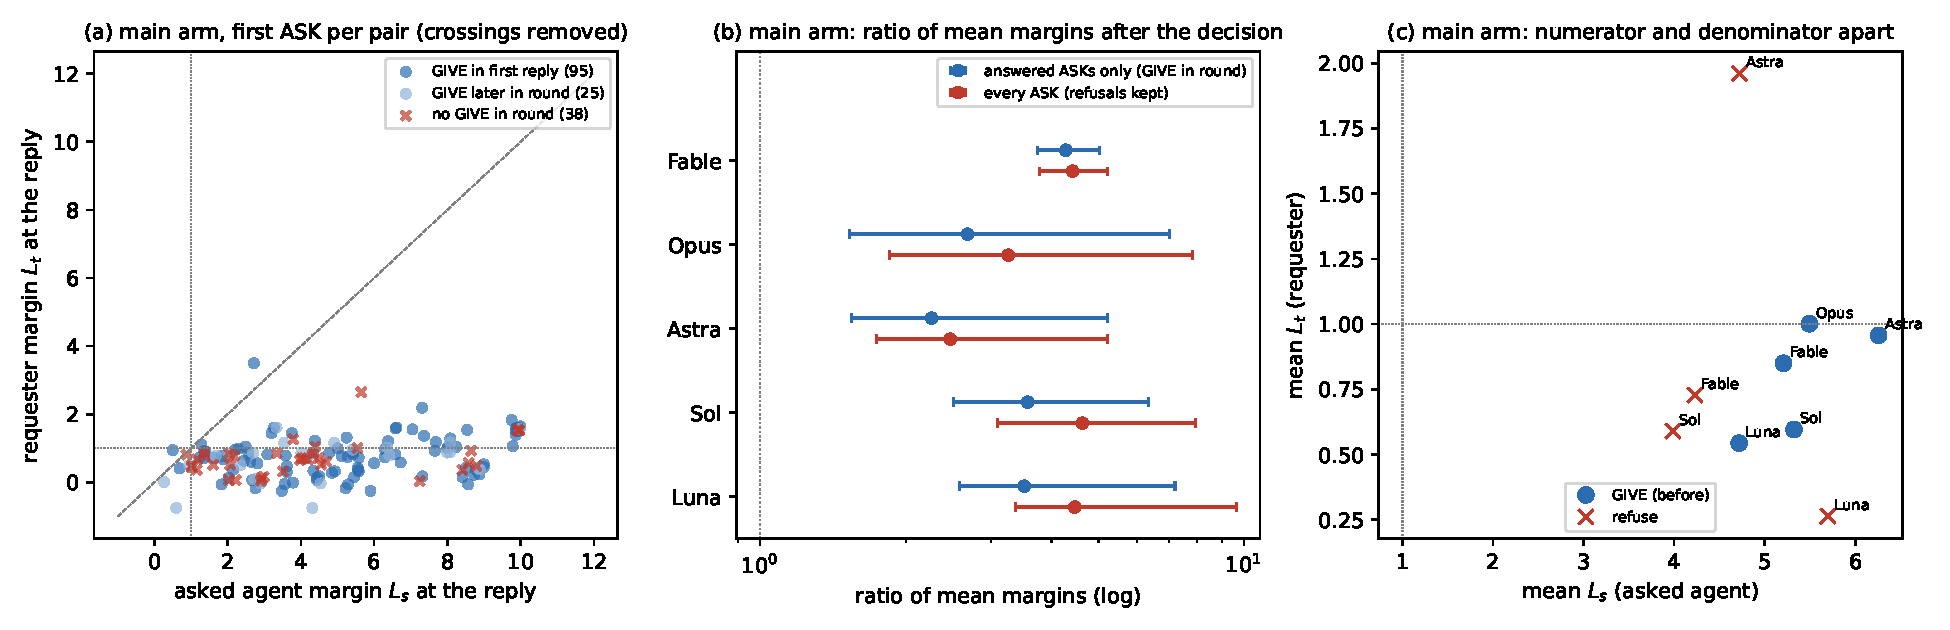
\includegraphics[width=\linewidth]{cogsci2027/validation_20261108/figures/w11_ask_refusal.pdf}
\caption{ASK 뒤 결정의 양쪽 여유(본 실험 2,000만 나눔, 교차한 요청 제외). (a) 첫 ASK마다 결정 직전 요청받은 쪽(가로)과 요청한 쪽(세로)의 생존 여유. 진한 파랑은 첫 응답의 GIVE, 옅은 파랑은 같은 라운드의 지연 GIVE, 빨간 X는 라운드 안 GIVE가 없던 거절이다. 점선은 $L=1$과 두 여유가 같은 선이며, 축 범위 밖의 값은 끝에 모았다. (b) 응답된 ASK만 쓴 $\rho_{\mathrm{GIVE}}$(파랑)와 거절을 포함한 $\rho_{\mathrm{all}}$(빨강), 시드 블록 부트스트랩 95\% 구간. (c) 모델별로 수락(결정 직전)과 거절의 평균 $L_s$와 평균 $L_t$를 따로 표시했다. Astra와 Luna의 거절은 각 2건이다.}
\label{val:w11-fig}
\end{figure}

\subsection{범위와 남는 한계}\label{val:w11-limits}

이 절의 표본은 ASK가 있었던 결정에 한정된다. 요청 없이 위기에 놓인 동료를 돕지 않은 선택, 자연어로만 도움을 청한 경우는 세지 않았다. 부록의 지원 기회 분석(절~\ref{app:aid-opportunities})은 확정 벌금에 부족한 수혜자와 예상 응답 비용까지 맞춘 더 좁은 기회를 정의했고, 그 77기회와 이 절의 471결정은 서로 다른 질문에 답한다. 거절을 라운드 끝까지 GIVE가 없던 결정으로 정의했으므로, 첫 응답에서 주지 않은 지연 지원 53건은 수락으로 셌다. 결정 뒤 상태는 응답 비용을 빼지 않은 장부 계산이며, 응답 비용은 수락과 거절 모두에 생긴다. 판과 결정은 같은 시드 안에서 서로 의존하므로 독립 표본으로 세지 않았고, 열 시드 블록만으로 구간을 냈다. 모든 비교는 결과를 본 뒤 정한 사후 분석이다.

\FloatBarrier
